\chapter{Introduction}

Cyber security systems are expected to monitor large volumes of network traffic continuously and identify malicious behaviour before it affects confidentiality, integrity or availability. Intrusion Detection Systems provide this monitoring layer by observing traffic features and classifying behaviour as normal or suspicious. Conventional software-based IDS pipelines can achieve strong detection performance, but they usually depend on dense numerical processing on general-purpose processors. This project studies an alternative neuromorphic IDS workflow where network traffic features are converted into spikes and prepared for processing through Leaky Integrate-and-Fire neuron circuits.

\section[Background]{\textbf{Background}}

Networked computing has expanded from desktop and server environments to mobile devices, cloud infrastructure, industrial control systems, smart sensors and Internet of Things deployments. As a result, the attack surface of a typical organization is no longer limited to a small number of managed machines. Attacks such as denial of service, reconnaissance, exploitation, worm activity, shellcode injection and generic malware traffic may appear as abnormal packet rates, unusual flow durations, uncommon protocol states, or suspicious byte-count patterns. An IDS attempts to identify such patterns from network observations.

Traditional IDS approaches can be broadly classified into signature-based and anomaly-based methods. Signature-based systems search for known malicious patterns and are effective when the attack database is complete. However, they are weak against new or modified attacks. Anomaly-based systems model normal behaviour and raise alerts when traffic deviates from that behaviour. Machine learning based IDS methods improve anomaly detection by learning relationships between traffic features and labels from historical datasets. These methods include Support Vector Machines, decision trees, Random Forests, neural networks and deep learning models \cite{Buczak2016}.

While machine learning improves adaptability, its computational style is usually dense and synchronous. Feature vectors are processed using repeated arithmetic operations, and the classifier is evaluated even when the input activity is low. This is acceptable in high-performance servers but less attractive for energy-constrained edge devices. A low-power IDS that can remain active continuously is useful for campus gateways, IoT hubs, industrial nodes and embedded network monitors. Neuromorphic computing is relevant in this context because it represents information through sparse spike events and performs computation primarily when events occur.

\section[Project Overview]{\textbf{Project Overview}}

The project titled \textbf{Neuromorphic Intrusion Detection System using Spiking Neural Networks and Leaky Integrate-and-Fire Neurons} is an interdisciplinary effort combining Information Science and Engineering with Electronics and Communication Engineering. The ISE component focuses on dataset handling, preprocessing, dimensionality reduction, spike encoding and classifier integration. The ECE component focuses on circuit-level compatibility, LIF neuron behaviour and SPICE/Cadence-ready waveform generation. The interface between these two components is the Piecewise Linear voltage source file.

The proposed system begins with the UNSW-NB15 network intrusion dataset. The raw dataset is cleaned, categorical values are encoded, numerical values are normalized and Principal Component Analysis is applied to reduce the processed feature space to a limited number of physical neuron inputs. The reduced analog feature values are then converted into spike trains using rate coding, time-to-first-spike coding or population coding. Finally, the spike trains are exported as PWL voltage files that can be directly applied to analog LIF neuron circuits.

\begin{table}[H]
\centering
\caption{Interdisciplinary team contribution structure}
\label{tab:teamstructure}
\begin{tabular}{|p{0.28\textwidth}|p{0.52\textwidth}|}
\hline
\textbf{Domain} & \textbf{Primary project contribution} \\
\hline
Information Science and Engineering & Dataset preprocessing, feature engineering, PCA reduction, spike encoding scripts, classifier integration and software workflow design. \\
\hline
Electronics and Communication Engineering & LIF neuron circuit understanding, analog waveform interpretation, Cadence/LTSpice simulation interface and hardware-oriented validation planning. \\
\hline
Common interdisciplinary interface & PWL waveform files that connect Python-generated IDS spike data with analog neuron circuit simulation. \\
\hline
\end{tabular}
\end{table}

\begin{figure}[H]
\centering
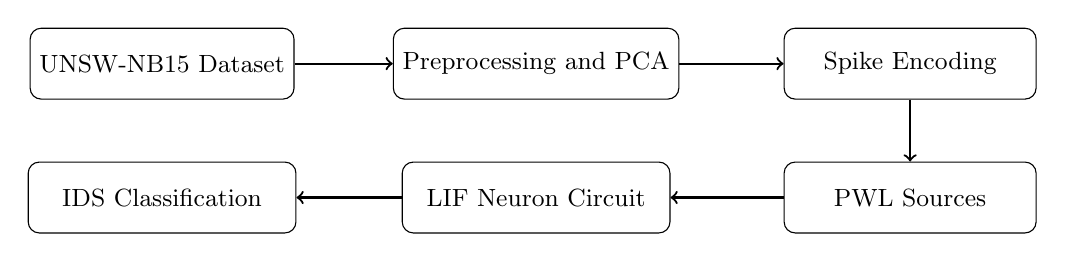
\begin{tikzpicture}[node distance=1.25cm, every node/.style={font=\small}]
\node[draw, rounded corners, minimum width=3.3cm, minimum height=0.9cm] (dataset) {UNSW-NB15 Dataset};
\node[draw, rounded corners, right of=dataset, xshift=3.5cm, minimum width=3.5cm, minimum height=0.9cm] (pipeline) {Preprocessing and PCA};
\node[draw, rounded corners, right of=pipeline, xshift=3.5cm, minimum width=3.2cm, minimum height=0.9cm] (spike) {Spike Encoding};
\node[draw, rounded corners, below of=spike, yshift=-0.45cm, minimum width=3.2cm, minimum height=0.9cm] (pwl) {PWL Sources};
\node[draw, rounded corners, left of=pwl, xshift=-3.5cm, minimum width=3.4cm, minimum height=0.9cm] (lif) {LIF Neuron Circuit};
\node[draw, rounded corners, left of=lif, xshift=-3.5cm, minimum width=3.4cm, minimum height=0.9cm] (classify) {IDS Classification};
\draw[->, thick] (dataset) -- (pipeline);
\draw[->, thick] (pipeline) -- (spike);
\draw[->, thick] (spike) -- (pwl);
\draw[->, thick] (pwl) -- (lif);
\draw[->, thick] (lif) -- (classify);
\end{tikzpicture}
\caption{High-level project workflow from dataset to neuromorphic IDS processing}
\label{fig:overallworkflow}
\end{figure}

Figure \ref{fig:overallworkflow} shows the conceptual workflow. The project is not limited to classifier training; it creates a hardware-facing representation of network traffic. The generated PWL files are a key output because they allow the same IDS samples processed in Python to be applied as voltage stimuli to a Cadence or SPICE neuron circuit.

\section[Literature Review]{\textbf{Literature Review}}

Intrusion detection has been studied extensively using statistical, machine learning and deep learning approaches. Moustafa and Slay introduced the UNSW-NB15 dataset to provide a modern benchmark containing normal network behaviour and multiple attack categories \cite{Moustafa2015}. The dataset includes flow-level attributes such as duration, protocol, service, source and destination byte counts, packet counts, time-to-live values, connection state and attack category. It is therefore suitable for training and testing IDS models.

Buczak and Guven surveyed data mining and machine learning techniques for cyber security intrusion detection and highlighted the importance of feature engineering, classifier selection and evaluation metrics \cite{Buczak2016}. Conventional IDS models can perform well when trained with representative data, but their deployment cost depends on the number of features, model complexity and frequency of inference. This is an important consideration for always-on detection systems.

Dimensionality reduction is commonly applied when datasets contain many correlated features. Principal Component Analysis transforms a feature matrix into orthogonal components ordered by variance contribution. Jolliffe and Cadima describe PCA as a fundamental method for reducing dimensionality while preserving dominant information in the dataset \cite{Jolliffe2016}. In this project, PCA is used not only for computational convenience but also to map a high-dimensional network feature space onto a limited number of analog neuron inputs.

Spiking Neural Networks represent a different computational paradigm. Maass described SNNs as the third generation of neural network models because they use spike timing as an additional computational dimension \cite{Maass1997}. Gerstner and Kistler formalized spiking neuron models, including membrane potential dynamics, threshold firing and reset behaviour \cite{Gerstner2002}. The LIF neuron is especially relevant for this project because it is simple enough to implement using analog circuit blocks while retaining the essential behaviour of spike generation.

Neuromorphic computing research aims to exploit event-driven processing for energy-efficient inference. Roy, Jaiswal and Panda discuss the potential of spike-based machine intelligence for neuromorphic hardware \cite{Roy2019}. Tavanaei et al. review deep learning in SNNs and discuss spike encoding strategies that convert continuous data into spike trains \cite{Tavanaei2019}. These studies motivate the idea that network traffic features can be transformed into spike-domain representations and processed using neuron-inspired hardware.

The gap addressed by this project lies between software IDS and circuit-level neuromorphic implementation. Many IDS projects stop at software classification, while many neuron circuit projects demonstrate isolated neuron behaviour without an application-specific data pipeline. This work attempts to connect both sides by preparing real IDS data as circuit-compatible spike stimuli.

Sommer and Paxson discuss the practical difficulties of applying machine learning to intrusion detection, especially the difference between controlled datasets and real operational environments \cite{Sommer2010}. Their observations are relevant to this work because the project avoids claiming that a classifier alone solves IDS deployment; instead, it focuses on building a hardware-compatible representation that can later be validated under controlled and realistic traffic settings.

Liao et al. survey IDS techniques and emphasize that network intrusion detection requires attention to feature representation, classification method and deployment constraints \cite{Liao2013}. This supports the project decision to treat preprocessing and representation design as first-class parts of the system rather than as minor steps before classification.

Diehl and Cook demonstrate that spiking neural networks can be trained and evaluated for pattern recognition tasks, showing that spike-based representations can support useful classification behaviour \cite{Diehl2015}. Although their work is not specific to IDS, it supports the broader feasibility of spike-domain information processing. Ponulak and Kasinski review supervised learning methods for SNNs and highlight the importance of spike timing, encoding and learning rules \cite{Ponulak2011}. These concepts are relevant to the spike feature extraction plan in this project.

Indiveri et al. describe neuromorphic silicon neuron circuits and show how neuron dynamics can be represented using physical circuit behaviour \cite{Indiveri2011}. This supports the ECE-side motivation of using LIF neuron circuits rather than limiting the project to a software-only SNN model. The literature collectively suggests that the project should be evaluated not only as an IDS classifier but as a complete representation-and-hardware workflow.

\begin{table}[H]
\centering
\caption{Summary of reviewed literature and relevance to the project}
\label{tab:litreview}
\begin{tabular}{|p{0.24\textwidth}|p{0.3\textwidth}|p{0.3\textwidth}|}
\hline
\textbf{Reference area} & \textbf{Main contribution} & \textbf{Relevance to this project} \\
\hline
UNSW-NB15 dataset \cite{Moustafa2015} & Provides modern labelled IDS traffic records. & Used as the project dataset. \\
\hline
ML for cyber IDS \cite{Buczak2016} & Reviews data mining and ML detection methods. & Supports the software IDS baseline workflow. \\
\hline
PCA \cite{Jolliffe2016} & Explains dimensionality reduction using principal components. & Used to map dataset features to limited neuron inputs. \\
\hline
SNN theory \cite{Maass1997,Gerstner2002} & Introduces spike-based computation and neuron models. & Provides foundation for spike-domain IDS representation. \\
\hline
Neuromorphic computing \cite{Roy2019,Indiveri2011} & Discusses event-driven hardware and neuron circuits. & Supports the hardware-oriented LIF design direction. \\
\hline
Spike encoding and SNN learning \cite{Tavanaei2019,Ponulak2011,Diehl2015} & Reviews spike encoding, SNN training and pattern recognition. & Supports rate, TTFS and population coding choices. \\
\hline
IDS deployment concerns \cite{Sommer2010,Liao2013} & Discusses practical IDS constraints and method selection. & Motivates a full workflow beyond classifier accuracy. \\
\hline
\end{tabular}
\end{table}

\section[Motivation]{\textbf{Motivation}}

The motivation of this project is not only to detect attacks but to study how attack-detection information can be represented in a neuromorphic form. A conventional IDS classifier works on numerical feature vectors. A neuromorphic IDS must convert those vectors into spike trains, process them through neuron dynamics and still retain useful information for classification. If this transformation is successful, it creates a path toward low-power security monitoring hardware.

The project is also motivated by interdisciplinary learning. The ISE team members contribute knowledge of datasets, preprocessing, machine learning and Python implementation. The ECE team members contribute knowledge of analog circuit behaviour, SPICE/Cadence simulation and LIF neuron design. A successful project requires a clean interface between these domains. In this project, that interface is the generated PWL waveform file.

\section[Problem Statement]{\textbf{Problem Statement}}

The problem addressed in this project is the design and implementation of a neuromorphic intrusion detection workflow that converts network traffic records into spike-based voltage waveforms and prepares them for LIF neuron processing. The system must preserve dataset labels, reduce the high-dimensional feature space into a practical number of hardware inputs, generate circuit-compatible PWL sources and provide a path for spike-feature extraction and IDS classification.

\section[Objectives]{\textbf{Objectives}}

The objectives of the project are:
\begin{enumerate}
\item To study the use of neuromorphic computing concepts for network intrusion detection.
\item To preprocess the UNSW-NB15 dataset by cleaning, encoding, normalizing and reducing the feature space.
\item To map processed network features into an analog-neuron-compatible representation using PCA.
\item To implement spike encoding methods that generate binary spike trains from normalized feature values.
\item To export spike trains as PWL voltage source files suitable for SPICE/Cadence LIF neuron simulation.
\item To define the software-hardware interface required for future extraction of LIF output spike features.
\end{enumerate}

\section[Expected Contributions]{\textbf{Expected Contributions}}

The expected contributions of the work documented in this report are:
\begin{enumerate}
\item A reproducible preprocessing pipeline for converting UNSW-NB15 records into normalized analog feature vectors.
\item A PCA-based mapping strategy that reduces high-dimensional IDS features to a fixed number of neuron inputs.
\item Multiple spike encoding methods implemented in Python for IDS feature conversion.
\item A PWL waveform generation method that allows direct use of encoded IDS samples in SPICE/Cadence voltage sources.
\item A documented interface between software-generated spike data and analog LIF neuron circuits.
\item A modular code structure that can be extended for waveform parsing, spike feature extraction and final IDS evaluation.
\end{enumerate}

\section[Scope of the Report]{\textbf{Scope of the Report}}

This report covers the project foundation, theoretical background, system design and implementation workflow. It includes the data pipeline, PCA-based feature reduction, spike encoding, PWL generation and the planned LIF circuit interface. It intentionally excludes detailed final results and final conclusion chapters because those are outside the requested report scope. Therefore, Chapters 5 and 6 are not included in this report.

\section[Brief Methodology]{\textbf{Brief Methodology}}

The methodology begins with dataset acquisition and preprocessing. Raw UNSW-NB15 CSV files are loaded, cleaned and converted into a numerical feature matrix. The attack category is retained as the label, while non-essential identifiers are removed. Min-Max scaling is applied before PCA. The PCA outputs are again scaled to the range 0 to 1 so that they can be interpreted as bounded analog values.

The normalized analog features are passed to a spike encoder. Rate coding, time-to-first-spike coding and Gaussian population coding are implemented. Population coding expands each feature into multiple receptive field responses. Each spike train is translated into a PWL waveform with time-voltage pairs. These PWL files are stored sample-wise and can be attached to voltage sources in circuit simulators.

The LIF circuit receives the PWL waveform as input. The membrane node integrates incoming activity, leakage reduces stored potential over time and the comparator output generates a spike when the membrane voltage crosses threshold. The output waveform can later be parsed to extract spike count, spike timing and firing rate features. These features can be used by a classifier to evaluate IDS performance.

\section[Assumptions and Constraints]{\textbf{Assumptions and Constraints}}

The project is based on the following assumptions:
\begin{enumerate}
\item The UNSW-NB15 dataset is representative enough for academic IDS experimentation.
\item PCA-reduced components retain sufficient information to represent traffic behaviour.
\item A limited physical neuron count requires dimensionality reduction before circuit mapping.
\item Normalized values in the range 0 to 1 can be converted into voltage-domain spike representations.
\item The LIF neuron is a suitable first neuron model because it is circuit-realizable and mathematically interpretable.
\end{enumerate}

The main constraints are:
\begin{enumerate}
\item Full hardware scaling requires multiple LIF circuit instances or time-multiplexed operation.
\item Circuit-level simulation time increases as the number of samples and input sources increases.
\item PWL files must be carefully formatted to avoid simulator convergence issues.
\item The report scope is limited to Chapters 1 to 4 and does not present final experimental results.
\end{enumerate}

\section[Organization of the Report]{\textbf{Organization of the Report}}

The report is organized as follows:
\begin{itemize}
\item Chapter 1 introduces the project, literature background, motivation, problem statement, objectives, methodology and scope.
\item Chapter 2 explains the theoretical fundamentals required for IDS preprocessing, spike encoding and LIF neuron modelling.
\item Chapter 3 presents the proposed system design, architecture, data flow, module design and validation strategy.
\item Chapter 4 describes the implementation details of the data pipeline, spike encoder, PWL file generation and hardware interface.
\end{itemize}
